\documentclass[11pt,a4paper]{article}

\usepackage[margin=1in]{geometry}
\usepackage{microtype}
\usepackage{amsmath,amssymb,amsthm,mathtools}
\usepackage{booktabs}
\usepackage{array}
\usepackage{graphicx}
\graphicspath{{charts/}{./}}
\usepackage{xcolor}
\usepackage{hyperref}
\usepackage[round,authoryear]{natbib}
\hypersetup{colorlinks=true,linkcolor=blue!60!black,urlcolor=blue!60!black,citecolor=blue!60!black}

\theoremstyle{plain}
\newtheorem{theorem}{Theorem}
\newtheorem{proposition}{Proposition}
\newtheorem{lemma}{Lemma}
\newtheorem{definition}{Definition}
\theoremstyle{remark}
\newtheorem{remark}{Remark}

\title{How Many Remain at Scale $\varepsilon$?\\
{\large The Dimensional Focal Point of a Corpus Point Map,\\ its Projection to the PCA Sphere, and the Deployed Map under its own Diagnostics}}
\author{Shant Tchatalbachian}
\date{November 10, 2026 (v1) --- revised November 10, 2026 (v2: live-deployment diagnostics)}

\emergencystretch=3em
\begin{document}
\maketitle

\begin{abstract}
Three short exchanges (2026-11-07) asked one question in three registers: cardinality, measure, summation and resolution are different kinds of ``infinity''; for data in an $N$-dimensional vector space, how many \emph{distinguishable} elements remain at scale $\varepsilon$ and at dimension $N$? This paper answers the question for a real, deployed object --- point map \#598 of the steady-orbit console, a frozen-frame \texttt{pointmap/0.2} map of the harness experience library --- and turns the answer into an automatic rule. (i) \textbf{Recovery.} The map's $3{,}232$ inputs are recovered exactly from its stored per-axis margins; re-running the repository instrument reproduces the stored \texttt{frame\_id}, \texttt{instrument\_id} and \texttt{run\_fingerprint}. The inputs are binary: the corpus lives on the vertices of $\{0,1\}^9$. (ii) \textbf{Four sizes.} The same corpus has $3{,}232$ items, $135$ distinct patterns, $116$ classes distinguishable by the deployed bit rule, and a Rényi spectrum $D_0/D_1/D_2=7.077/6.606/6.265$ bits; on a binary cube at lattice resolution, $\log_2 N$ \emph{is} an effective dimension. (iii) \textbf{The dimensional focal point.} Keeping only projection axes that add at least half a bit of distinguishability at lattice scale selects $n^\star=7$ for every Rényi order, robustly for any threshold in $(0.055,0.722)$ bits. The knee is set by marginals --- two primitives are present in $98.7\%$ and $99.8\%$ of items, and both fixed-margin nulls reproduce it --- while the residual is the corpus's own: the eighth axis adds $0.055$ bit against $0.340\pm0.026$ under the curveball null ($z=-11.0$), and at $n^\star$ the information and collision dimensions sit $15.2$ and $12.3$ null SDs below chance. (iv) \textbf{Certified resolution.} Using the instrument's own half-space certificates (kernel-checked in \texttt{WayfinderBounds}), most of the $37$ classes contributed by the two discarded axes cease to be certifiably distinct under an $\ell_\infty$ input perturbation of $0.014$ ($1.4\%$ of the unit input range). (v) \textbf{Projection to the PCA sphere.} The focal coordinates are lifted to $S^2$ with the program's own pipeline; the stereographic scale is identified as the lens power of the series' Möbius chart, and the RMS rescale already used by the curved-corpus program attains at least $95\%$ of the best resolved count on both globes, while the deployed \texttt{0.9/maxR} rule under-powers the focal globe by a factor $2.4$ and roughly halves its resolved count. The focal globe keeps all $135$ patterns and is more faithful to the focal geometry (Spearman $0.438$ vs $0.314$), but resolves fewer positions at the canonical chord $0.095$ ($61$ vs $79$); the trade-off is reported, not resolved. (vi) \textbf{The real maps under the live diagnostics.} The six instruments of the console's Map card $\to$ diagnostics sub-tab were run against the live deployment with operator authentication, and from repository source. The API stores three maps. As deployed on 2026-11-10, the live record of \#598 equalled the recovered map (margins identical), and its three stored instruments reproduced exactly; the live maps have since been re-embedded in place with \texttt{bge-m3} (2026-11-12 and 2026-11-14), so the binary record now survives only in the archive. With the trial operating cap raised from $N\le1200$ to $N\le4000$ (\texttt{AXIS\_TRIAL\_MAX\_N}), all four HTTP trials run in full on the $N=3{,}232$ map as well as on the $1{,}200$-item subsample: on the smaller stored maps (\#595, \#596) and on the $d=7$, $1024$-D \texttt{bge-m3} map \#598 of 2026-11-12, live responses agree with repository source on all $4{,}461$ and $5{,}243$ returned fields (maximum numeric difference $4.0\times10^{-13}$). On the full binary \#598 ($N=3{,}232$), axis redundancy excludes all nine axes (total $z=61.6$; top two axes $9$ and $2$, with all nine $z\in[22.9,28.4]$), and admission admits \texttt{axis\_trial} and \texttt{spectra}. Applied to the $1024$-D \texttt{bge-m3} re-embeddings, the focal-probe refreeze rule ($d=n^\star$ from a $d_{\mathrm{probe}}$ scan; refreezing is idempotent by \texttt{focalDim\_refreeze\_fixed}) selects $d=\lfloor\log_2 N\rfloor$ on \#596 ($d=5$) and \#598 ($d=11$, $1{,}364$ classes vs.\ $128$ saturated codes at $d=7$), and $d=6<\lfloor\log_2 N\rfloor=7$ on \#595 ($N=135$). On every re-embedded map the selected $n^\star$ is not separable from the curveball null. The fixed $V_2\ge0.40$ gate ($\hat r=2/V_2\le5$) is kept as the \emph{dimension} readout, which marks the prefix at which a map can be focused, and \emph{structure} is read separately with the same statistic against a fixed-margin null at the same prefix; the two readouts are logically independent (\texttt{gate\_structure\_independent}). On the $1024$-D maps the focus dimension is $5$--$6$. There \#598 and the knowledge corpus are structured ($z=5.3$ and $6.6$; $0.15$ and $0.28$ effective dimensions below the null), while \#595 and \#596 pass the gate without structure resolved from the null. (vii) Twenty-seven exact identities --- refinement by one bit never merges classes and at most doubles them, $\le2^d$, the focal selection rule, and the sign and mutual independence of the dimension and structure readouts --- are proved in core Lean~4 and pass every gate of the series' CI.
\end{abstract}

\section{Introduction}
\label{sec:intro}

The curved-corpus program has measured corpora by their concentration ($V_2$), their curvature against matched nulls, their optics and their diffusion \citep{tch2026latent,tch2026isthisx,tch2026unified}. It has not yet asked the most elementary question one can ask of a finite map: \emph{how many things are on it?} The question is less trivial than it looks. On 2026-11-07 three short exchanges with a general-purpose assistant posed it in sequence. The first asked for the state of the art on a ``fluid'' transition between finite and infinite sets and received the standard decomposition: cardinality, measure, summation and resolution count different things, and the useful substitution is to replace exact membership by observational resolution --- ``ask how many distinguishable elements remain at scale $\varepsilon$''. The second carried the substitution to $\mathbb{R}^N$: packing and covering numbers $P_\varepsilon,C_\varepsilon\sim(L/\varepsilon)^N$, metric entropy $\log_2 C_\varepsilon\approx N\log_2(L/\varepsilon)$, and, for constrained data, an effective (box-counting) dimension in place of $N$. The third surveyed the mathematical theory of box-counting dimension. Those transcripts are the seed of this paper; their citations were independently re-verified before use (Section~\ref{sec:scope}), and one of their formulas is corrected below.

This paper does four things. It \textbf{recovers} a deployed map exactly and shows that its inputs are binary, which makes every count in the transcripts exact rather than asymptotic (Section~\ref{sec:data}). It \textbf{defines} a dimensional focal point --- the projection dimension at which a corpus is resolved, chosen automatically and null-standardized --- and applies it (Section~\ref{sec:focal}). It \textbf{projects} the focused map to the PCA sphere with the program's own pipeline and identifies the lift scale as the lens power of the series' optical reading (Section~\ref{sec:sphere}). And it \textbf{audits} every map stored on the deployment with the console's own diagnostics tab, on the live API and from source (Section~\ref{sec:diag}). Counting identities are machine-checked (Section~\ref{sec:lean}); scope and caveats close.

The disciplines of the 2026-08-12 paper \citep{tch2026isthisx} are inherited verbatim: no statistic without its matched null, no coordinate admitted without a non-degenerate null, verdicts are exclusion-only, and every number is quoted from a stored artifact.

\section{Four sizes of a finite corpus}
\label{sec:sizes}

Let $X=\{x_1,\dots,x_M\}\subset\mathbb{R}^D$ be a corpus with multiplicities and $\pi_n$ the projection onto its top-$n$ principal axes. Four quantities are in play.

\begin{definition}[Sizes]
\emph{Cardinality} $M$ (items, with multiplicity); \emph{distinct count} $|\{x_i\}|$; \emph{resolution count} $N(\varepsilon,n)$, the size of a maximal $\varepsilon$-separated subset of $\pi_n(X)$ (a packing; the greedy construction used here is maximal, hence bracketed by covering numbers, $C_\varepsilon\le N(\varepsilon,n)\le C_{\varepsilon/2}$, \citealp{kolmogorov1959entropy}); and the \emph{measure-weighted} sizes $2^{D_q}$, where $D_q(\varepsilon,n)$ is the Rényi entropy of order $q$ of the item distribution over the cells of that packing,
\begin{equation}
D_0=\log_2(\#\text{cells}),\qquad D_1=-\sum_c p_c\log_2p_c,\qquad D_2=-\log_2\sum_c p_c^2 .\tag{1}
\end{equation}
\end{definition}

$D_0$ counts, $D_1$ weights by measure, $D_2$ is a collision (correlation) count; they are the finite-scale members of the generalized-dimension family \citep{hentschel1983infinite,grassberger1983characterization} and satisfy $D_2\le D_1\le D_0$. For a finite set every box-counting dimension is $0$ in the limit $\varepsilon\to0$ \citep{falconer2014fractal}; dimension is therefore a property of a \emph{scale window}, which is exactly the transcripts' point that infinity becomes ``a scale-dependent growth law''.

\paragraph{A correction to the seed formula.} The second exchange counts the $\varepsilon$-grid of $[0,L]^N$ as $(\lceil L/\varepsilon\rceil+1)^N$; the number of grid points with spacing $\varepsilon$ in $[0,L]$ is $\lfloor L/\varepsilon\rfloor+1$, and the asymptotic $C_\varepsilon\sim P_\varepsilon\sim(L/\varepsilon)^N$ hides $N$-dependent constants ($\log C_\varepsilon=N\log(L/\varepsilon)+O(N\log N)$), which matter at $N$ of embedding size. Neither affects what follows, because on a binary cube the lattice count is exact:

\begin{proposition}[Lattice resolution on the cube]
\label{prop:cube}
If $X\subseteq\{0,1\}^d$ and $\varepsilon<1$, distinct points are $\varepsilon$-separated in the Euclidean metric, so $N(\varepsilon,d)=|\{x_i\}|$ and $D_0=\log_2|\{x_i\}|\le d$, with equality iff every vertex is occupied. Hence $D_0$ at lattice resolution is an effective dimension in bits, and the per-axis gain $\Delta D_0(n)=D_0(n)-D_0(n-1)$ is the number of bits the $n$-th axis contributes.
\end{proposition}

\paragraph{Related work.} Packing and box-counting dimension go back to the metric-entropy programme of \citet{kolmogorov1959entropy} and to the packing measures of \citet{tricot1982two}; textbook treatments are \citet{falconer2014fractal}, \citet{mattila1995geometry} and \citet{federer1969geometric}. Three lines are directly relevant here. (i) \emph{Projections:} box and packing dimensions are not preserved by orthogonal projection, and their almost-sure values under projection are governed by dimension profiles \citep{falconer1996projection,falconer1997packing}; the focal rule is an empirical, finite-scale analogue, which asks how many projection axes a finite corpus needs before further axes stop adding resolution. (ii) \emph{Interpolation between dimensions:} intermediate dimensions \citep{falconer2020intermediate}, the dimension spectra of \citet{fraser2018new}, Minkowski dimension for measures \citep{falconer2023minkowski} and the survey of \citet{fraser2026invitation} all replace a single exponent by a profile over scales. That is the stance taken here, where dimension is read off a scale window rather than a limit. (iii) \emph{Intrinsic dimension in machine learning:} estimators based on packing numbers \citep{kegl2002intrinsic}, nearest-neighbour likelihood \citep{levina2004maximum}, two-nearest-neighbour ratios \citep{facco2017estimating} and correlation sums \citep{grassberger1983characterization} are reviewed by \citet{camastra2016intrinsic}. Random projections preserve pairwise distances up to $1\pm\epsilon$ in $O(\epsilon^{-2}\log M)$ dimensions \citep{dasgupta2003elementary}, and effective data dimensionality controls the learning rates of kernel regression \citep{zhang2005learning}. The first exchange's ``fluid'' passage from finite to infinite through hyperfinite sets is the province of non-standard analysis \citep{robinson1966nonstandard}; it is not used here.

\section{The deployed map, recovered exactly}
\label{sec:data}

Map \#598 is stored in the console's KV namespace as \texttt{map-json:598} (5.37~MB). It is a \texttt{pointmap/0.2} frame (rule R0: frozen top-$d$ PCA axes, bit $b_j=[\,s_j>\mathrm{median}_j\,]$, then $z$-score, PCA-2 and stereographic lift to $S^2$) over $M=3{,}232$ items of the corpus \texttt{harness/experience-library} (knowledge, skills, docs, playbooks), with $d=D=9$, seed $20260906$, $K=200$ null draws.

The raw vectors are not stored, but every item's signed margin $m_{ij}=s_{ij}-\theta_j$ against each frozen threshold is (field \texttt{math\_diagnostics.per\_input}). Hence $s_{ij}=m_{ij}+\theta_j$ and $x_i=\mu+s_i^{\top}A$ with the stored orthonormal axes $A$ ($\|AA^{\top}-I\|_\infty=1.8\times10^{-15}$). Four checks make the recovery exact: the recomputed bits equal the stored bits on all $3{,}232\times9$ entries; the stored thresholds equal the sample medians of the recovered scores; the deployed placement applied to the recovered bits reproduces \texttt{pts\_full} to machine precision; and running the repository's unmodified \texttt{pointmap.js} on the recovered vectors reproduces \texttt{frame\_id} \texttt{77360296af046f8d}, \texttt{run\_fingerprint} \texttt{fba40c7b482d4e2e}, $V_2=0.39573$ and the null $z=70.36$. The recovered inputs take exactly two values per coordinate: \textbf{the corpus is a multiset on the vertices of $\{0,1\}^9$}, a nine-primitive coverage code like the program's $2286\times9$ matrix.

\begin{table}[h]\centering\small
\begin{tabular}{lr}
\toprule
size of map \#598 & value \\
\midrule
cardinality (items) & $3{,}232$ \\
distinct input patterns (of $512$) & $135$ \\
classes distinguishable by the deployed bit rule ($d=9$) & $116$ (largest $128$; $74{,}064$ unresolvable pairs) \\
distinct top-$d$ bit prefixes, $d=1,\dots,9$ & $2, 4, 8, 16, 30, 49, 79, 95, 116$ \\
Rényi $D_0/D_1/D_2$ of exact patterns (bits) & $7.077/6.606/6.265$ \\
Rényi $D_0/D_1/D_2$ of deployed classes (bits) & $6.858/6.399/6.109$ \\
\bottomrule
\end{tabular}
\caption{The four sizes of the same corpus. The deployed rule (rotate to PCA, then cut at medians) resolves $19$ fewer elements than the data contain even at full dimension, because median hyperplanes on rotated axes do not align with the facets of the cube. Source: recovered map \#598; \texttt{focal/numbers.json}.}
\label{tab:sizes}
\end{table}

\section{The dimensional focal point}
\label{sec:focal}

Proposition~\ref{prop:cube} turns the transcripts' question into a curve. Project the binary corpus onto its top-$n$ PCA scores, $n=1,\dots,9$, and count distinguishable cells at the lattice scale $\varepsilon_{\mathrm{lat}}=0.9$ (below the unit edge of the cube; above it, vertices merge). Each added axis either splits cells, contributing up to one bit, or does not.

\begin{definition}[Dimensional focal point]
\label{def:focal}
For a Rényi order $q$ and threshold $\tau$, the focal dimension is
\begin{equation}
n^\star_q(\tau)=\max\{\,n:\ \Delta D_q(n')\ge\tau\ \text{for all } n'\le n\,\},\qquad \Delta D_q(n)=D_q(\varepsilon_{\mathrm{lat}},n)-D_q(\varepsilon_{\mathrm{lat}},n-1),\tag{2}
\end{equation}
the largest prefix of axes each of which still adds at least $\tau$ bits. The default is $\tau=\tfrac12$ bit: an axis is kept if it at least halves the typical cell in the $q$-weighted sense. The rule is automatic --- no scale, no target count, and no label enters it.
\end{definition}

\begin{table}[h]\centering\small
\resizebox{\linewidth}{!}{%
\begin{tabular}{lccccccccc}
\toprule
axis $n$ & 1 & 2 & 3 & 4 & 5 & 6 & 7 & 8 & 9 \\
\midrule
$\Delta D_0(n)$, real & 1.585 & 1.000 & 0.737 & 1.000 & 0.722 & 0.956 & 1.000 & 0.055 & 0.022 \\
$\Delta D_1(n)$, real & 1.100 & 1.002 & 0.842 & 0.939 & 0.694 & 0.928 & 1.063 & 0.031 & 0.007 \\
$\Delta D_0(n)$, curveball mean ($K=20$) & 1.585 & 1.029 & 0.768 & 0.692 & 0.841 & 1.084 & 0.990 & 0.340 & 0.057 \\
\bottomrule
\end{tabular}}
\caption{Bits contributed by each PCA axis at lattice scale. The first seven axes each add at least $0.722$ bit; the eighth and ninth add $0.055$ and $0.022$. Under the margin-preserving curveball null the knee is also at seven, but the eighth axis adds $0.340$ bit.}
\label{tab:gains}
\end{table}

\paragraph{Result.} With $\tau=\tfrac12$, $n^\star_0=n^\star_1=n^\star_2=7$ (Table~\ref{tab:gains}, Figure~\ref{fig:focal}). The choice is stable for every $\tau\in(0.055,0.722)$ bits for $D_0$ and $(0.031,0.694)$ for $D_1$, which together cover two orders of magnitude of threshold. The reason is visible in the loadings: axes $8$ and $9$ carry variances $0.0125$ and $0.0018$ against $\ge0.1449$ for the others, and load $0.98$ and $0.98$ on two input primitives that are present in $98.7\%$ and $99.8\%$ of items ($43$ and $7$ items lack them). The remaining seven primitives occupy all $2^7=128$ of their joint patterns, and at $n^\star$ the lattice count is exactly $N(\varepsilon,7)=128$ for every $\varepsilon\in[0.074,0.942]$ --- a plateau that is descriptive, not the selection criterion.

\paragraph{Null standardization.} The knee itself is a property of the marginals: both fixed-margin nulls, the curveball chain \citep{carstens2015}, as used in the 2026-08-12 paper \citep{tch2026isthisx}, and an independent column permutation, also select $n^\star=7$. What is \emph{not} a property of the marginals is how little the corpus does beyond the knee and how unevenly it fills the focal cube:
\begin{itemize}
\item the eighth axis adds $0.055$ bit against $0.340\pm0.026$ (curveball, $K=20$, $z=-11.0$) and $0.342\pm0.021$ (column permutation, $K=50$, $z=-13.4$): the rare primitives co-occur with patterns that already exist instead of creating new ones;
\item at $n^\star=7$, $D_0/D_1/D_2=7.000/6.568/6.240$ against null $6.990/6.634/6.334$ ($z=+2.3/-15.2/-12.3$): every cell is occupied, but the occupancy is far more concentrated than the marginals imply;
\item at $n=9$ the corpus has $135$ distinct patterns against $167.5$ (curveball) and $168.9$ (column permutation); $D_0$ $z=-12.4$.
\end{itemize}
The focal point thus separates two things the deployed map conflates: \emph{how many dimensions the corpus uses} ($n^\star=7$, a marginal fact) and \emph{how it uses them} (strongly non-random, $z\approx-12$ to $-15$).

\begin{figure}[t]\centering
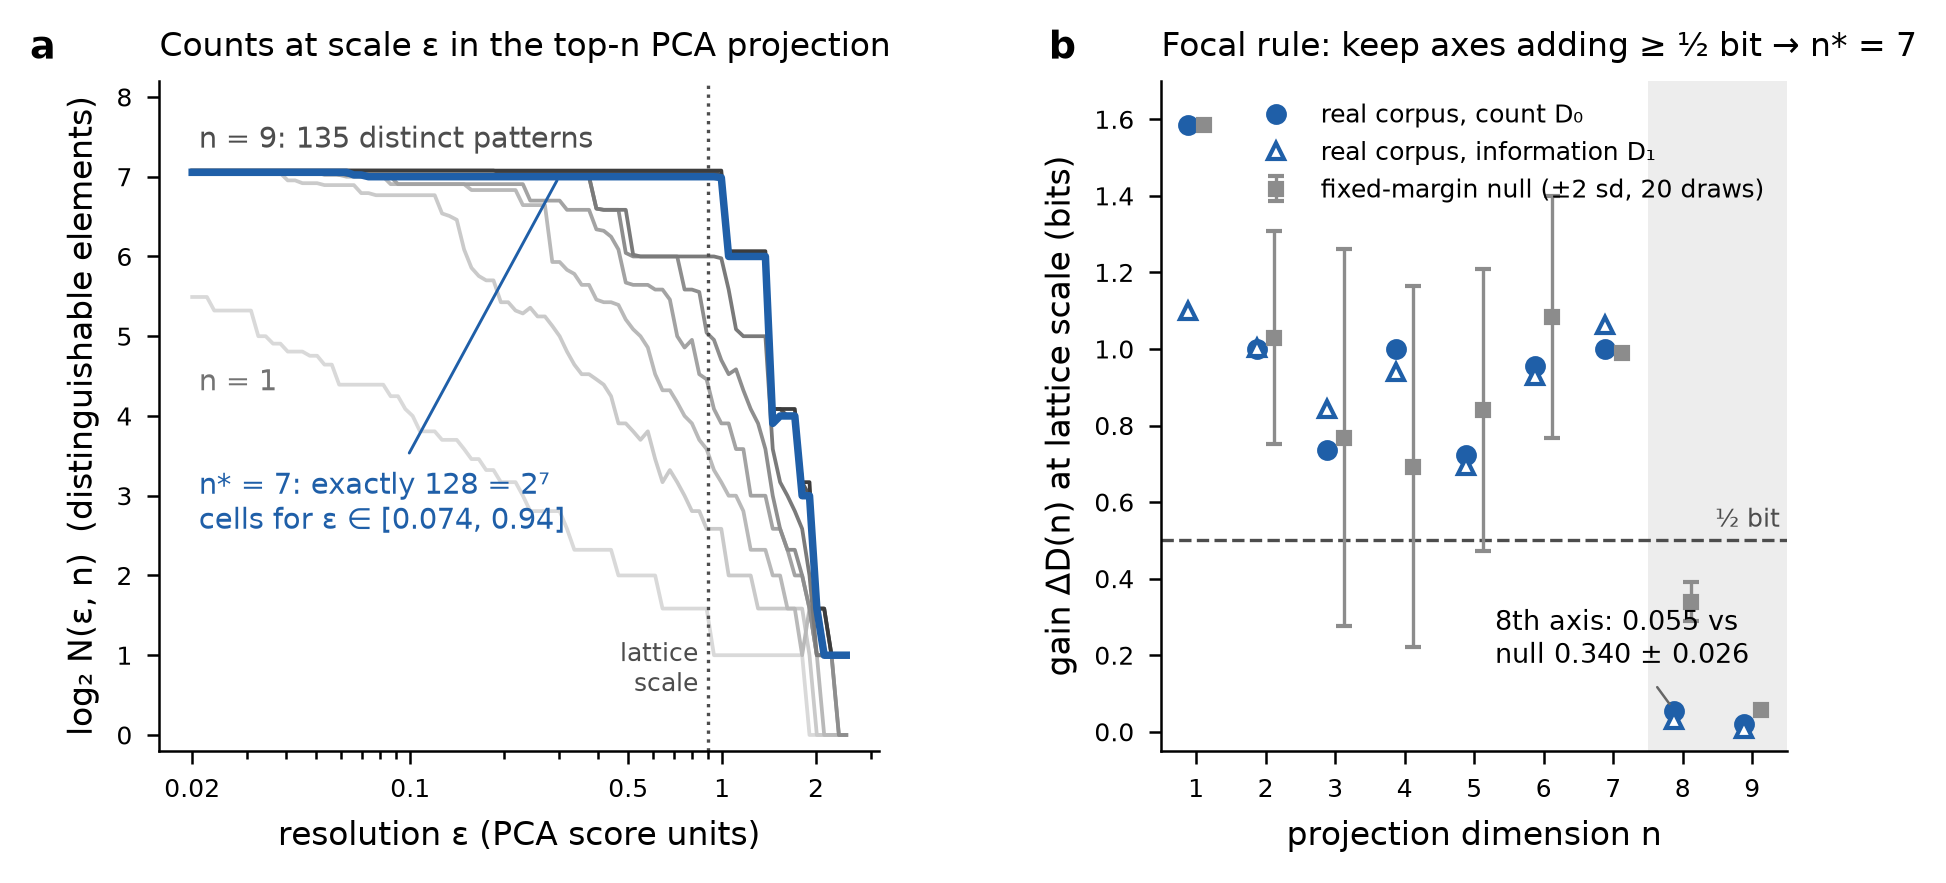
\includegraphics[width=\linewidth]{dfp_fig1_distinguishability.png}
\caption{Distinguishability versus resolution and dimension. (a) $\log_2N(\varepsilon,n)$ in the top-$n$ PCA projection for $n=1,\dots,9$; the dotted line is the lattice scale $\varepsilon_{\mathrm{lat}}=0.9$, and at $n^\star=7$ the count is exactly $128=2^7$ on $[0.074,0.94]$. (b) Per-axis gain $\Delta D_0$ (filled) and $\Delta D_1$ (open) against the fixed-margin curveball null (mean $\pm2$~sd, $20$ draws); axes in the shaded band fall below the $\tfrac12$-bit rule. Source: \texttt{renyi.npz}.}
\label{fig:focal}
\end{figure}

\section{Certified distinguishability}
\label{sec:certified}

The deployed instrument distinguishes items by signs of margins $m_{ij}$. The series' \texttt{WayfinderBounds} module proves that a half-space verdict is stable under any perturbation $\delta$ with $|\langle a,\delta\rangle|<|m|$ (lemmas \texttt{stable\_on}/\texttt{stable\_off}); for $\|\delta\|_\infty\le\varepsilon$ this holds whenever $|m_{ij}|>\varepsilon\|a_j\|_1$. Call two classes \emph{certifiably distinct at $\varepsilon$} if they differ on a bit whose margin is certified for both items. A greedy maximal family of pairwise certifiably distinct classes gives a lower bound on the robust class count.

\begin{table}[h]\centering\small
\begin{tabular}{lcccccc}
\toprule
$\varepsilon$ & 0.0000 & 0.0016 & 0.0137 & 0.0568 & 0.0721 & 0.0914 \\
\midrule
$d=9$ (deployed) & 114 & 94 & 77 & 53 & 44 & 37 \\
$d=7=n^\star$ & 77 & 76 & 69 & 49 & 44 & 37 \\
\bottomrule
\end{tabular}
\caption{Lower bounds on certifiably distinct classes under an $\ell_\infty$ input perturbation $\varepsilon$ (greedy, hence lower bounds). The median $|m|$ on axes $8$ and $9$ is $0.0240$ and $0.0017$, against $0.32$--$0.46$ on axes $1$--$7$.}
\label{tab:cert}
\end{table}

At $\varepsilon=0$ the two discarded axes contribute $37$ extra classes; by $\varepsilon=0.0137$ only $8$ remain, and the two curves meet near $\varepsilon\approx0.07$ (Figure~\ref{fig:cert}). The classes the focal rule discards are, for the most part, the classes a $1.4\%$ perturbation of the input would erase.

\begin{figure}[t]\centering
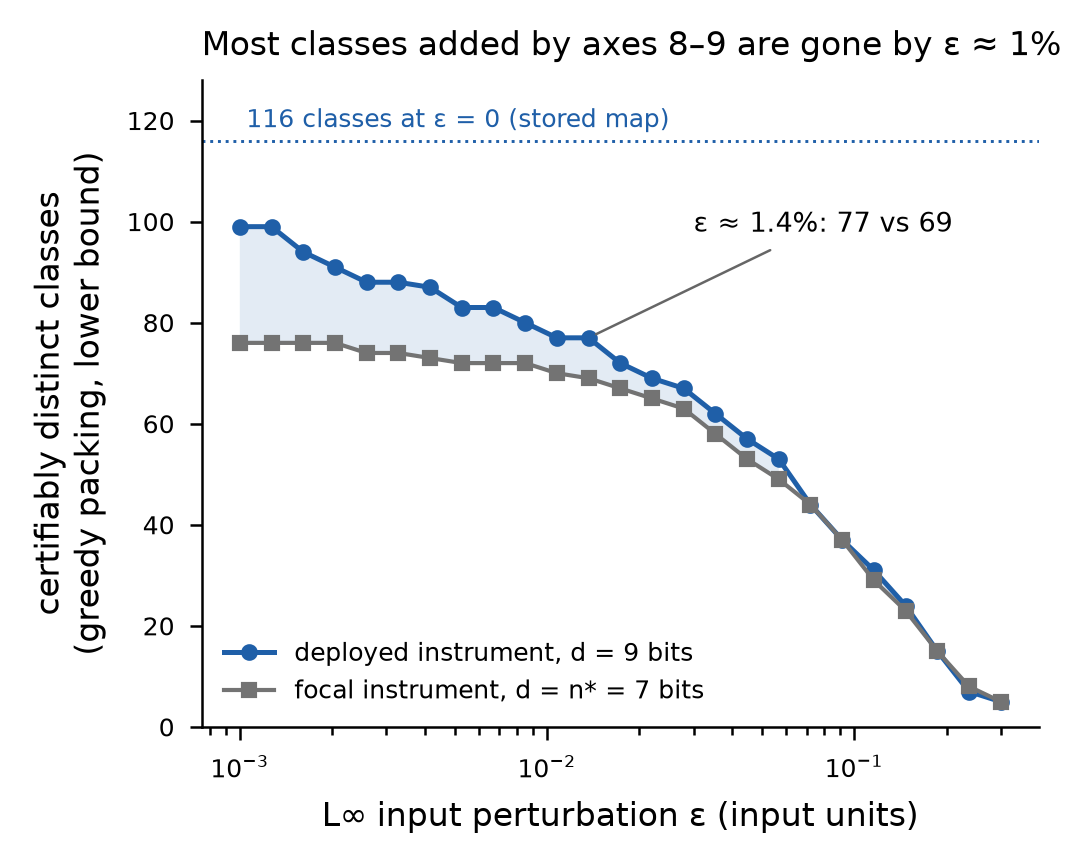
\includegraphics[width=0.8\linewidth]{dfp_fig2_certified.png}
\caption{Certified class counts (greedy lower bounds) at $d=9$ and $d=n^\star=7$ versus $\ell_\infty$ input perturbation, on a logarithmic axis from $\varepsilon=10^{-3}$. The dotted line is the $116$ classes of the stored map; at $\varepsilon=0$ the strict-margin certificate gives $114$ and $77$ (Table~\ref{tab:cert}). The shaded gap is the contribution of axes $8$--$9$; at $\varepsilon=0.0137$ it is $77$ vs $69$. Source: \texttt{robust.npz}.}
\label{fig:cert}
\end{figure}

\section{Projection to the PCA sphere}
\label{sec:sphere}

The focal coordinates are mapped to $S^2$ with the program's own placement: $z$-score, PCA-2 and the stereographic lift $(u,v)\mapsto\big(2su,2sv,1-s^2r^2\big)/(1+s^2r^2)$, $r^2=u^2+v^2$. The \emph{focal globe} places the continuous top-$n^\star$ scores; the \emph{deployed globe} places the $9$ bits. The top two PCs of the focal coordinates carry $28.6\%$ of their variance.

\paragraph{Lens power.} For points of the plane, $s$ acts as a dilation, and dilation by $s$ composed with inverse stereographic projection is a Möbius transformation of $S^2$; $s$ is therefore the power of the series' Möbius lens. Three powers are compared: the deployed rule $s=0.9/\max r$, the RMS rescale $s=1/\mathrm{RMS}(r)$ of the curved-corpus paper, and the focal power $s^\star$ that maximizes $N(0.095)$, the number of positions distinguishable at the canonical chord used by every diagnostic of the console.

\begin{table}[h]\centering\small
\begin{tabular}{lccccccc}
\toprule
globe & distinct & \multicolumn{3}{c}{$N(0.095)$ at $s=$} & $N(0.02)$ & isolated & Spearman $\rho$ \\
 & positions & $0.9/\max r$ & RMS & $s^\star$ & & & vs focal \\
\midrule
deployed (bits, $d=9$) & 116 & 75 & 79 & 80 & 94 & 2 & 0.314 \\
focal ($n^\star=7$ scores) & 135 & 33 & 61 & 64 & 133 & 0 & 0.438 \\
\bottomrule
\end{tabular}
\caption{The two globes. Powers: deployed $s=0.34/0.53/0.75$, focal $s=0.38/0.71/0.90$ (maxR/RMS/$s^\star$). Spearman correlation of chord distances with distances in the seven-dimensional focal space, on a fixed random subsample of pairs. Isolated: positions with no neighbour within chord $0.095$.}
\label{tab:globes}
\end{table}

The trade-off is genuine and is reported rather than resolved. The deployed globe resolves more positions at $0.095$ ($79$ vs $61$ at RMS power), because bits are well-separated by construction. The focal globe keeps every one of the $135$ input patterns as a distinct position, preserves the focal geometry better ($\rho=0.438$ vs $0.314$), and resolves $133$ positions at chord $0.02$ against $94$. The RMS rescale attains $99\%$ and $95\%$ of the best count on the two globes; the deployed $0.9/\max r$ rule attains $52\%$ on the focal globe, because a few outlying patterns set $\max r$. RMS is therefore the recommended automatic power.

\begin{figure}[t]\centering
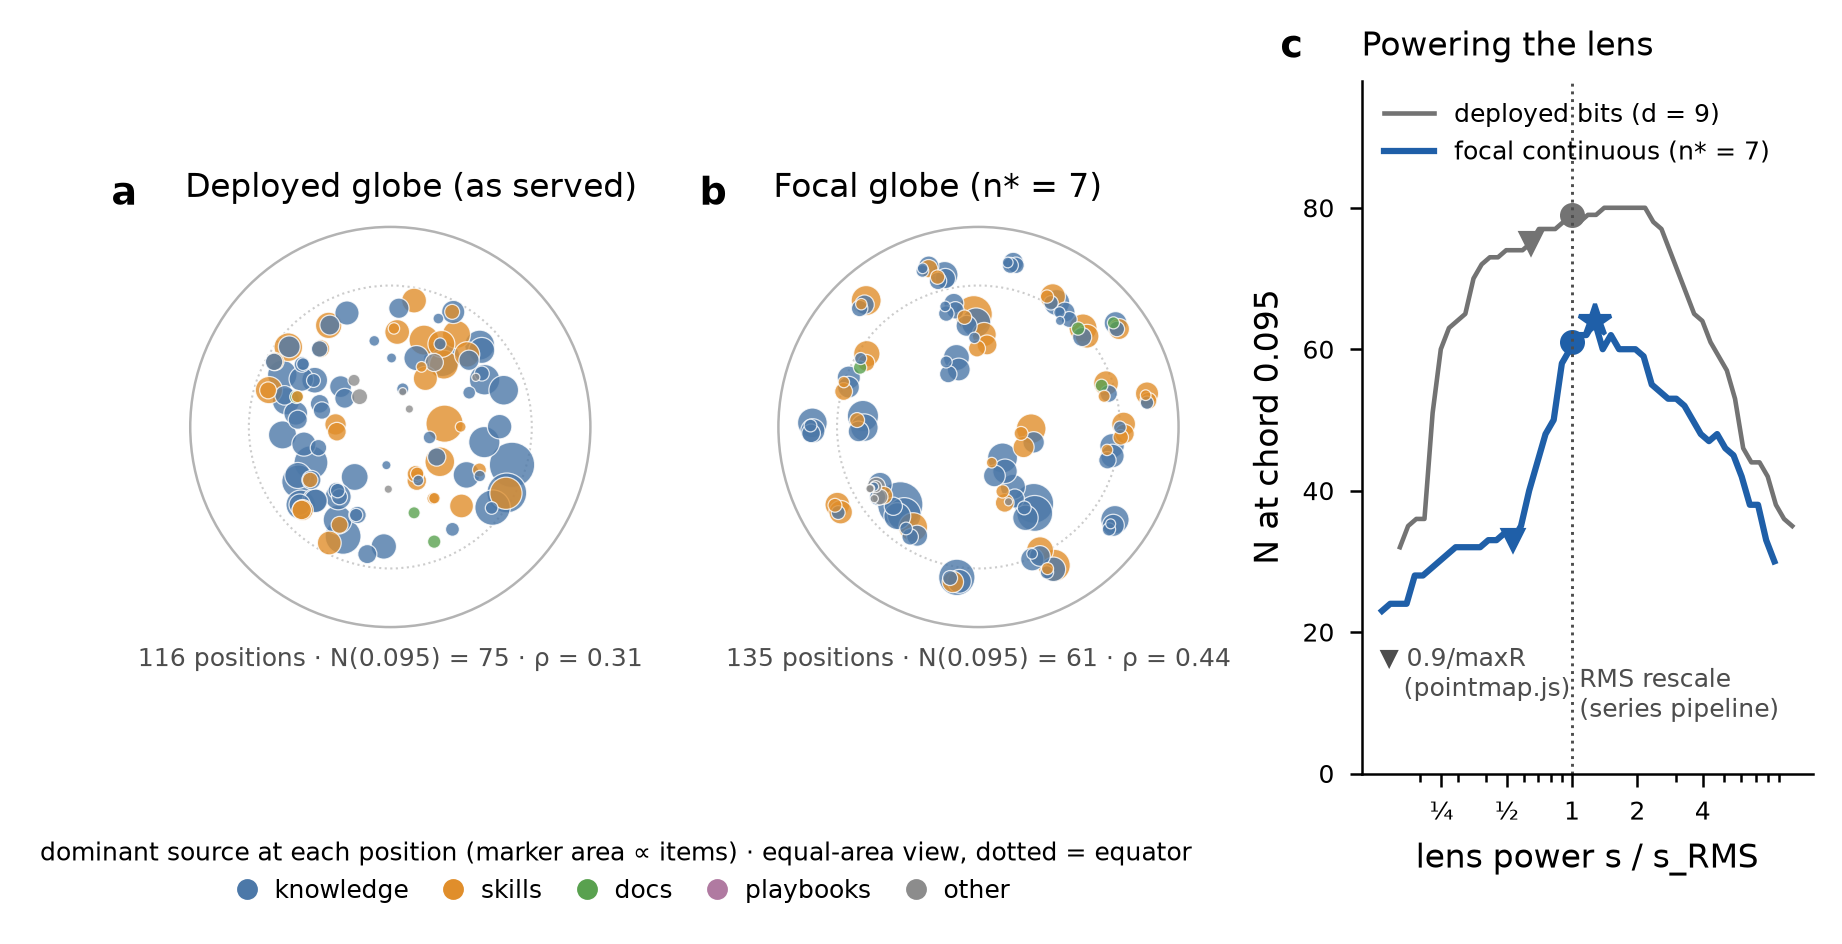
\includegraphics[width=\linewidth]{dfp_fig3_pca_sphere.png}
\caption{Projection to the PCA sphere. (a) The deployed globe as served ($s=0.9/\max r$). (b) The focal globe at RMS lens power. Markers show the dominant corpus section at each position, area proportional to items; equal-area view, dotted circle the equator; $\rho$ is the Spearman correlation with seven-dimensional focal distances. (c) $N(0.095)$ against lens power $s/s_{\mathrm{RMS}}$ for both globes; $\blacktriangledown$ marks $0.9/\max r$, $\bullet$ the RMS rescale and $\star$ the best power $s^\star$. Source: \texttt{lens\_scan.npz}, \texttt{globes.npz}.}
\label{fig:sphere}
\end{figure}

\section{The real map under its own diagnostics}
\label{sec:diag}

The console's Map card has a diagnostics sub-tab that drives six instruments: spectroscopy, radius profile and the $V_2$ null, which are computed at map time and stored with the map, and four HTTP trials (\texttt{/api/jev/map/\{azimuth, rayleigh, admission, axis-redundancy\}}). All six were run from repository source (\texttt{tools/point-map}) against map \#598 and the $d=n^\star$ re-map, and the four trials were also run against the live deployment (\texttt{steady-orbit} worker, 2026-11-10) with the operator bearer key. The live listing \texttt{GET /api/jev/map/maps} returns three maps. The map fold rewrites that path to the \texttt{/api/maps} handler, which in the deployed source selects every row with no \texttt{LIMIT} or pagination, and the live response carries exactly that query's 15 columns. The three maps are \#598 (\texttt{harness/experience-library}, $n=3{,}232$, $D=9$), \#596 (\texttt{policy/jev-policy.json}, $n=52$, $D=768$, \texttt{bge-base} text embeddings) and \#595 (\texttt{harness/skills}, $n=135$, $D=768$). The live record of \#598 has the stored \texttt{frame\_id} and \texttt{run\_fingerprint}, and its per-item margins equal the recovered ones exactly (maximum absolute difference $0$). It differs from the KV backup only in that the read path decodes the compact \texttt{margin-tuples/1} storage encoding.

\paragraph{Parity.} The three stored instruments reproduce the stored map exactly: spectroscopy, radius profile and null agree with maximum absolute difference $0$.

\paragraph{Operating range of the four trials: subsample ($N=1{,}200$) and full map ($N=3{,}232$).} The trials are $O(N^2dK)$. In the initial 2026-11-10 deployment \texttt{AXIS\_TRIAL\_MAX\_N} was $1{,}200$, so \#598 was first evaluated on a seeded $1{,}200$-item subsample (mulberry32, seed $20261110$). Raising \texttt{AXIS\_TRIAL\_MAX\_N} to $4{,}000$ (commit \texttt{0af108e6}) enabled all four trials to run on the full $N=3{,}232$ binary map from repository source and on the live $d=7$, $1024$-D \texttt{bge-m3} map \#598 of 2026-11-12 (frame \texttt{5272393cca0ca74b}) over the API (where all $5{,}243$ returned fields across azimuth, rayleigh, admission and axis redundancy match repository source to within $4.0\times10^{-13}$). Table~\ref{tab:diag} reports both the $N=1{,}200$ subsample and the full $N=3{,}232$ map side by side.

\paragraph{The live trials on the stored maps that fit.} Maps \#595 and \#596 are below the cap, so all four trials run in full on the live endpoint (Table~\ref{tab:live}). Repository source, run on the live map records, returns the same results on every one of the 4{,}461 fields of the eight responses, with identical field sets and a maximum numeric difference of $1.9\times10^{-14}$ (float round-off). For the diagnostics code path, the deployment and the repository are therefore equivalent on every map the deployment can run.

\begin{table}[h]\centering\small
\resizebox{\linewidth}{!}{%
\begin{tabular}{lcc}
\toprule
 & \#595 \texttt{harness/skills} & \#596 \texttt{policy} \\
\midrule
$N$ (all items; no subsample) & $135$ & $52$ \\
rayleigh components (null mean $\pm$ sd) & $88$ ($89.1\pm4.71$) & $36$ ($44.2\pm2.59$) \\
rayleigh $z$ / isolates (null mean) & $-0.23$ / $60$ ($59.9$) & $-3.16$ / $25$ ($37.4$) \\
axis redundancy: excluded axes (total $z$) & $2,7$ ($3.26$) & $3,4,5,6,8$ ($4.58$) \\
axis-trial admission blocked by & seed reproducibility & seed reproducibility, $N<100$ \\
admitted: rayleigh, axis, spectra, radius, azimuth & T, F, T, T, F & F, F, F, F, F \\
\bottomrule
\end{tabular}}
\caption{The four live trials on the two stored maps below the cap (live endpoint, operator key, default $K=40$). Every value equals the repository-source result. Azimuth is not admitted on either map: its de-atomized null is not size-matched and its Holm verdicts are not reproducible across seeds.}
\label{tab:live}
\end{table}

\paragraph{The focal rule on every stored map.} Definition~\ref{def:focal} needs only a ladder of distinguishable counts, so it applies to the deployed bits of every map. The top-$d$ bit-prefix count is the $D_0$ ladder of the instrument itself, and its gains are exact by \texttt{FocalBounds} ($N_d\le N_{d+1}\le2N_d$). The null is a curveball chain on each map's bit matrix ($20$ draws, $100n$ trades), which preserves the near-balanced median-split columns.

\begin{table}[h]\centering\small
\resizebox{\linewidth}{!}{%
\begin{tabular}{lcccccccccccc}
\toprule
map ($n$) & \multicolumn{9}{c}{$\Delta D_0(d)$ of the bit ladder, $d=1,\dots,9$} & $n^\star$ & null $n^\star$ & $\log_2 n$ \\
\midrule
\#598 ($3{,}232$) & 1.000 & 1.000 & 1.000 & 1.000 & 0.907 & 0.708 & 0.689 & 0.266 & 0.288 & $7$ & $9$ & $11.66$ \\
\#595 ($135$) & 1.000 & 1.000 & 1.000 & 1.000 & 0.954 & 0.746 & 0.585 & 0.254 & 0.216 & $7$ & $6$--$7$ & $7.08$ \\
\#596 ($52$) & 1.000 & 1.000 & 1.000 & 0.807 & 0.716 & 0.334 & 0.312 & 0.152 & 0.170 & $5$ & $5$--$6$ & $5.70$ \\
\bottomrule
\end{tabular}}
\caption{The focal rule ($\tau=\tfrac12$ bit) on the deployed bit ladder of each stored map. Ladders: \#598 2, 4, 8, 16, 30, 49, 79, 95, 116; \#595 2, 4, 8, 16, 31, 52, 78, 93, 108; \#596 2, 4, 8, 14, 23, 29, 36, 40, 45. Class counts at $d=9$ against the null: \#598 $z=-160.5$, \#595 $z=-4.8$, \#596 $z=-4.4$.}
\label{tab:focalmaps}
\end{table}

On \#598 the bit ladder independently gives $n^\star=7$, the same focal point as the lattice rule of Section~\ref{sec:focal}. At the bit level the knee is corpus-specific: the null on the balanced deployed bits fills every axis ($n^\star=9$), and the real map has $116$ classes against a null mean of $504$. On \#595 and \#596 the rule returns $n^\star=7$ and $5$, but their nulls return $6$--$7$ and $5$--$6$. With $n=135$ and $52$ items the ladder cannot exceed $\log_2 n=7.08$ and $5.70$ bits, so the rule meets the sample ceiling before it meets the corpus. These two maps are too small to have an identifiable focal point. That is the finite-size face of the paper's question: how many dimensions remain distinguishable is bounded by how many items there are to distinguish.

\begin{table}[h]\centering\small
\resizebox{\linewidth}{!}{%
\begin{tabular}{lcccc}
\toprule
 & deployed $d=9$ (sub $1{,}200$) & deployed $d=9$ (full $3{,}232$) & focal re-map $d=7$ & focal globe$^\dagger$ \\
\midrule
spectroscopy $E_{0..3}$ & 0.42/0.25/0.06/0.27 & 0.42/0.25/0.06/0.27 & 0.44/0.38/0.01/0.17 & 0.70/0.05/0.21/0.05 \\
even / odd & 0.481/0.519 & 0.481/0.519 & 0.453/0.547 & 0.905/0.095 \\
radius: isolated at $r=0.075\ldots0.115$ & 3,2,2,2,2 & 3,2,2,2,2 & 0,0,0,0,0 & 0,0,0,0,0 \\
rayleigh comp / isol / largest & 73 / 4 / 58 (109.6) & 75 / 2 / 161 (106.3) & 71 / 2 / 75 (97.9) & 47 (---) \\
axis redundancy: excluded (total $z$; top-2) & 9/9 ($33.8$; $9,8$) & 9/9 ($61.6$; $9,2$) & 7/7 ($16.2$) & --- \\
admitted: rayleigh, axis, spectra, radius, azimuth & T, T, F, T, F & F, T, T, F, F & T, T, T, F, F & --- \\
\bottomrule
\end{tabular}}
\caption{The diagnostics sub-tab on the binary map \#598: seeded $1{,}200$-item subsample vs.\ full $N=3{,}232$ map (\texttt{AXIS\_TRIAL\_MAX\_N = 4000}), alongside the $d=7$ focal re-map and focal globe$^\dagger$. T/F: admitted / not admitted.}
\label{tab:diag}
\end{table}
\begin{figure*}[t]
\centering
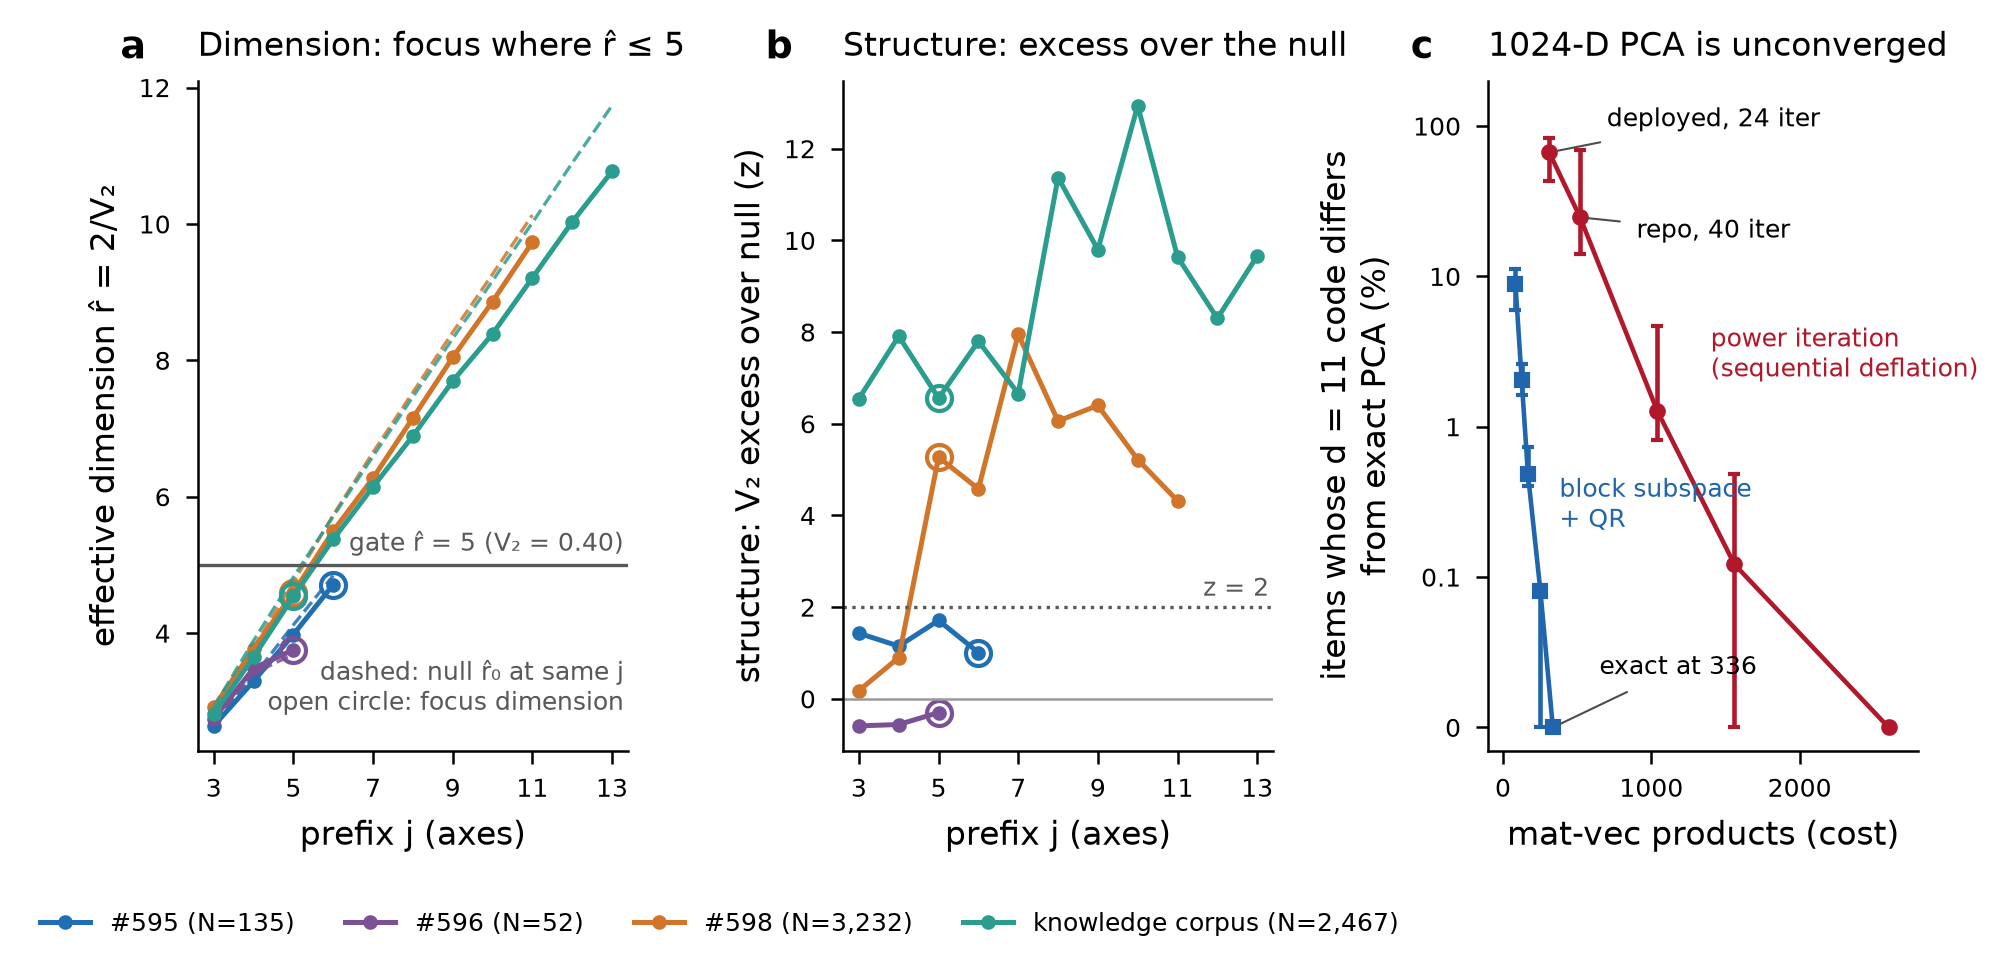
\includegraphics[width=\linewidth]{dfp_fig4_gate_pca.png}
\caption{Dimension, structure and the frame on $1024$-D \texttt{bge-m3} maps. (a) Dimension: effective dimension $\hat r=2/V_2$ of each prefix code (solid) and of a curveball null on the same prefix (dashed, $\hat r_0$); the fixed gate $\hat r\le5$ ($V_2\ge0.40$) marks the focus dimension (open circles). (b) Structure: excess of $V_2$ over that null, $z=(V_2-\mu_0)/\sigma_0$ ($K=20$). \#595, \#596 and \#598 are the live 2026-11-14 records; the knowledge corpus ($N=2{,}467$) is mapped at $d=13$ on a block-PCA frame. (c) Fraction of knowledge-corpus items whose $d=11$ code differs from exact PCA, against the number of matrix--vector products, for sequential power iteration with deflation ($24$--$200$ iterations) and block subspace iteration with QR ($4$--$16$ steps, $k=13$, $8$ oversampling vectors); median and range over $8$ seeds; $0$ plotted at the axis floor.}
\label{fig:gate}
\end{figure*}

\paragraph{What the tab sees (subsample vs.\ full map, and Option 1 vs.\ Option 2 refreeze on 1024-D \texttt{bge-m3}).} Five readings matter. (1) \emph{Axis redundancy on the full map.} All nine axes remain excluded ($z=61.6$ at $N=3{,}232$ vs.\ $33.8$ on the subsample), but while the subsample ranked axes $9$ and $8$ first, on the full map the top two are $9$ and $2$ (axis $8$ is sixth, with all nine per-axis $z$ tightly grouped in $22.9$--$28.4$), showing that individual axis-redundancy ranks are not a robust witness for the knee. (2) \emph{Full-map admission flips.} At $N=3{,}232$ \texttt{rayleigh} ($75$ components, $2$ isolates, $112{,}126$ edges) is no longer admitted, because its isolates null is degenerate ($0$ isolates in all $40$ draws of one seed) and that verdict flips between seeds; \texttt{radius\_profile} fails on a degenerate null; and \texttt{spectra} is admitted alongside \texttt{axis\_trial}. (3) \emph{Azimuth} remains unadmitted ($Z_2,Z_3,Z_4$ excluded). (4) \emph{Focal re-map.} The $d=7$ re-map removes all isolated positions ($0$ vs.\ $3$) and passes spectroscopy admission. (5) \emph{Option 1 ($d=\lfloor\log_2 N\rfloor$) vs.\ Option 2 (focal-probe refreeze at $d=n^\star$) on 1024-D \texttt{bge-m3} text embeddings.} When maps \#595, \#596 and \#598 are embedded in $1024$-D (\texttt{@cf/baai/bge-m3}), $d=7$ saturates on \#598 ($128/128$ codes). Option~2 probes up to $d_{\mathrm{probe}}=\min(24,\lfloor\log_2 N\rfloor+2)$ and refreezes at $d=n^\star$ (idempotent by \texttt{focalDim\_refreeze\_fixed}). Both rules select $d=5$ on \#596 ($N=52$) and $d=11$ on \#598 ($N=3{,}232$, $1{,}364$ classes) and on the $2{,}467$-document \texttt{yubi-OS/knowledge} corpus ($1{,}166$ classes); on \#595 ($N=135$) Option~2 stops at $d=6$, where the seventh axis adds $0.47$ bit $<\tau=0.5$. Three qualifications apply (Fig.~\ref{fig:gate}). First, on every refrozen map the live focal trial returns \emph{not separable from the null}: the ladder is truncated at $d=n^\star$, and on the knowledge corpus the curveball null yields the same $n^\star=11$. Second, the $V_2\ge0.40$ gate and the $\hat r\le5$ rank gate are one test ($\hat r=2/V_2$ exactly). $V_2$ is the top-two eigenvalue share of a $d\times d$ bit-correlation matrix whose trace is $d$, so $\hat r$ is an effective dimension of the prefix code and grows with $d$ by construction. The gate therefore reads \emph{dimension}, the largest prefix at which the map can be focused, and is kept as such. Whether the code is more concentrated than its margins imply is a separate question, answered by the same statistic against a fixed-margin null at the same prefix (Section~\ref{sec:dimstruct}). In those terms \#595 passes the gate at $d=6$ ($\hat r=4.71$) as a dimension statement only, since its excess over the null is not resolved at any prefix, and \#598 fails the gate at $d=11$ ($\hat r=9.73$) while lying above its null. Third, for $D>40$ the frame's PCA axes come from seeded power iteration with sequential deflation, which is not converged at $D=1024$, where the eigenvalue ratios of axes $4$--$13$ are $0.89$--$0.94$. On the knowledge corpus, after the repository's $40$ iterations $14$--$70\%$ of items (median $25\%$, $8$ seeds) receive a different $d=11$ code than under exact PCA, and after the $24$ iterations the deployment now uses for $N>2000$, $D\ge512$, $43$--$83\%$ do; the $d=11$ class count ranges over $1{,}145$--$1{,}185$ and $1{,}136$--$1{,}159$ respectively, against $1{,}169$ exactly. The focal point itself is robust ($n^\star=11$ in every variant), but class membership, \texttt{frame\_id} and certificates on high-dimensional maps are seed- and solver-dependent. Block subspace iteration with QR ($k+8$ vectors, $16$ steps; $336$ matrix--vector products, against $312$ for $24$ power iterations) reproduces the exact codes on every seed.

\section{Dimension and structure}
\label{sec:dimstruct}

{\sloppy A prefix code answers two different questions, and the console reports both (\texttt{dimension-structure/1}, in the focal trial and on every stored map). \emph{Dimension.} With $V_2(j)$ the top-two eigenvalue share of the $j\times j$ correlation matrix of the first $j$ bits, $\hat r(j)=2/V_2(j)$ is the effective dimension of the prefix code. The fixed gate $V_2\ge0.40$, equivalently $\hat r\le5$ (\texttt{CurvedCorpus.gate\_rank\_identity}), is unchanged; the \emph{focus dimension} $d_{\mathrm{focus}}$ is the largest prefix that passes it, the deepest code whose two leading components still carry two fifths of its correlation. \emph{Structure.} At the same $j$, $V_2$ is compared with a curveball null on the $j$-bit prefix matrix (row and column sums preserved; $K=20$, $25N$ trades per draw): $\hat r_0(j)=2/\mathbb{E}_0[V_2]$ is the effective dimension the margins alone produce, $\Delta\hat r=\hat r_0-\hat r$ is the corpus's concentration in dimension units, and $z$ with an empirical two-sided tail decides whether it is resolved. $\Delta\hat r\ge0$ exactly when $V_2\ge\mathbb{E}_0[V_2]$ (\texttt{FocalBounds.structure\_sign\_identity}). Neither readout implies the other (\texttt{FocalBounds.gate\_structure\_independent}): independent fair bits at $j=3$ pass the gate with no structure, and twelve bits carrying two weak group factors fail it at $z=48$ (\texttt{test-dimension-structure.mjs}).\par}

\begin{table}[h]
\centering
\small
\begin{tabular}{lcccc>{\raggedright\arraybackslash}p{4.2cm}}
\toprule
 & $N$ & $d_{\mathrm{focus}}$ & $\hat r$ / $\hat r_0$ at $d_{\mathrm{focus}}$ & $z$ at $d_{\mathrm{focus}}$ & readout at the stored $d$ \\
\midrule
\#595 & $135$ & $6$ & $4.71$ / $4.84$ & $1.01$ & low-dimensional, not resolved from null ($d=6$) \\
\#596 & $52$ & $5$ & $3.76$ / $3.69$ & $-0.30$ & low-dimensional, not resolved from null ($d=5$) \\
\#598 & $3{,}232$ & $5$ & $4.59$ / $4.75$ & $5.27$ & structured, above focus ($d=11$) \\
knowledge & $2{,}467$ & $5$ & $4.54$ / $4.82$ & $6.56$ & structured, above focus ($d=13$) \\
\bottomrule
\end{tabular}
\caption{Dimension and structure on the $1024$-D \texttt{bge-m3} maps (live records of 2026-11-14) and the $2{,}467$-document knowledge corpus (block-PCA frame, $d=13$). Profiles over every prefix are in Fig.~\ref{fig:gate}a,b.}
\label{tab:dimstruct}
\end{table}

The focus dimension is $5$ or $6$ on every map, well below the focal point $n^\star$ ($11$ on \#598 and the knowledge corpus): the information ladder keeps paying past the depth at which a two-dimensional view summarises the code. On the two large corpora the focused code is structured beyond its margins, by $0.15$ and $0.28$ effective dimensions ($z=5.3$ and $6.6$), and the excess grows with $j$ ($\Delta\hat r=0.40$ at $d=11$ on \#598, $0.96$ at $d=13$ on the knowledge corpus). On \#595 and \#596 ($N=135$ and $52$) the gate passes but no prefix is resolved from the null. The null preserves row sums, so a factor shared by all bits is absorbed by it; the structure readout measures concentration beyond the margins, not all correlation.

\section{Machine-checked counting identities}
\label{sec:lean}

The counting facts used above are exact and finite, so they are proved, not estimated. A new module \texttt{FocalBounds.lean} (core Lean~4, toolchain $4.33.0$, no Mathlib) defines \texttt{distinctCount} on lists via an explicit \texttt{dedup}, the top-$d$ prefix count of a bit-code family, and the focal selection rule (Definition~\ref{def:focal}) on a gain list, and proves $27$ theorems:

\begin{theorem}[FocalBounds]
For a list of codes $c$ and every $d$:
{\sloppy
\begin{enumerate}
\item \texttt{distinctCount\_le\_length}, \texttt{distinctCount\_map\_le}: a map never has more classes than items, and any recoding cannot increase the class count;
\item \texttt{distinctCount\_perm}, \texttt{distinctCount\_congr}: class counts are invariant under reordering and under pointwise-equal codings;
\item \texttt{prefix\_count\_mono}, \texttt{prefix\_count\_double}: adding one bit never merges classes and at most doubles them, $N_d\le N_{d+1}\le2N_d$;
\item \texttt{prefix\_count\_pow}, \texttt{prefix\_count\_le\_length}: $N_d\le2^d$ and $N_d\le M$ (given codes of length $\ge d$);
\item \texttt{focalDim\_le\_length}, \texttt{focalDim\_prefix\_meets}, \texttt{focalDim\_stop\_fails}, \texttt{focalDim\_maximal}: the selected $n^\star$ is a prefix all of whose gains meet $\tau$, the next gain (if any) fails, and no longer such prefix exists;
\item \texttt{focalDim\_take\_self}, \texttt{focalDim\_refreeze\_fixed}: re-applying the focal rule to the $n^\star$ selected gains returns $n^\star$, so refreezing at $n^\star$ is idempotent;
\item \texttt{antitone\_stabilizes}, \texttt{recode\_stabilizes}: under any sequence of recodings the distinct count is non-increasing, so within $N_0$ steps, where $N_0$ is the initial distinct count, some step leaves the count unchanged. This is a plateau, not a fixed point: later steps may still merge classes.
\item \texttt{structure\_sign\_identity}, \texttt{gate\_structure\_independent}: with $V_2=p/q$ and null mean $E_0=r/s$, $V_2\ge E_0\iff 2s/r\ge 2q/p$, so the structure excess and $\Delta\hat r\ge0$ are one test; and rational witnesses show that the dimension gate and the structure excess are logically independent (Section~\ref{sec:dimstruct}).
\end{enumerate}\par}
\end{theorem}

Items 3 and 4 require a code-length premise, which the instrument's codes satisfy. The module passes every gate of the series' \texttt{lean-check} workflow: forbidden-token scan, no \texttt{sorry}, \texttt{leanchecker} replay, axiom coverage ($61$ constants, the $27$ theorems and $34$ auto-generated auxiliaries, all within the series' permitted core set \texttt{propext}, \texttt{Quot.sound}, \texttt{Classical.choice}; no \texttt{sorryAx}), a scope manifest (\texttt{FOCAL\_SCOPE\_MANIFEST\_OK 27}), the per-theorem axiom and statement pins ($27/27$) and negative controls (an injected \texttt{sorry}, a mutant with \texttt{distinctCount := 0} and a mutant that drops the inequality from \texttt{fracGe}, the last two leaving every statement unchanged, are all rejected). Run locally under the patched \texttt{lean-check} workflow, with \texttt{FocalBounds} added as a sixth module, all $57$ executed steps of \texttt{lean-check} and \texttt{lean-run} pass with $0$ failures (re-run 2026-11-14 with the two dimension/structure theorems), including the three focal steps (kernel check, scope-manifest validation, axiom pins) and the \texttt{leanchecker} replay of all six modules.

\section{Scope and honest caveats}
\label{sec:scope}

\begin{enumerate}
\item \textbf{One corpus, binary inputs.} Every result is about map \#598. Proposition~\ref{prop:cube} makes the counts exact precisely because the inputs are binary; for continuous embeddings the lattice scale must be replaced by an estimated one, and the focal rule becomes a choice of scale window \citep{falconer2014fractal,camastra2016intrinsic}.
\item \textbf{Subsample vs.\ full-map diagnostics.} Raising \texttt{AXIS\_TRIAL\_MAX\_N} from $1{,}200$ to $4{,}000$ (commit \texttt{0af108e6}) confirmed that three of five admission decisions and the top-two axis-redundancy ranks change between the $1{,}200$-item subsample and the full $N=3{,}232$ map (Table~\ref{tab:diag}); only full-map diagnostics should be used for admission decisions.
\item \textbf{Deployed equivalence is behavioural, not byte-level.} The four live trials agree with repository source (commits \texttt{7d095ae} and \texttt{0af108e6}) on all $4{,}461$ fields for \#595/\#596 and all $5{,}243$ fields for full $N=3{,}232$ \#598 (max diff $4.0\times10^{-13}$). That establishes behavioural equivalence of the diagnostics code path on the maps stored on 2026-11-12. The maps re-embedded on 2026-11-14 (\#598 at $d=11$, \#596 at $d=5$, \#595 at $d=6$) have not been re-checked, and the deployment now runs $24$ rather than $40$ power iterations when $N>2000$ and $D\ge512$, so on such maps deployed and repository frames differ.
\item \textbf{Two of three stored maps are small.} Maps \#595 and \#596 have $n=135$ and $52$, so their focal rule is sample-limited (Table~\ref{tab:focalmaps}). Only \#598 is large enough for the focal point to be a corpus property.
\item \textbf{Packings are lower bounds.} All $N(\varepsilon)$ above $\varepsilon_{\mathrm{lat}}$ and all certified counts are greedy, hence lower bounds on the packing number.
\item \textbf{Nulls.} Fixed-margin nulls control marginals only. Curveball draws use $K=20$ and column permutations $K=50$; $z$-scores are descriptive. Because row sums are preserved, a factor shared by all bits is absorbed by the null, so the structure readout of Section~\ref{sec:dimstruct} measures concentration beyond the margins.
\item \textbf{The focal rule has a free parameter.} $\tau=\tfrac12$ bit is a convention; the reported $n^\star$ holds across the whole stable band $(0.055,0.722)$.
\item \textbf{Literature.} The seed transcripts' citations were re-verified bibliographically (39 of 42 confirmed). Unconfirmed items, including Bouligand (1928), are not cited. The seed transcripts conflate two Falconer capacity papers, invert an author order, and misattribute a DOI; only corrected entries are used here.
\end{enumerate}

\section{Conclusion}

The answer to ``how many remain at scale $\varepsilon$'' for this corpus is a ladder --- $3{,}232$ items, $135$ patterns, $116$ deployed classes, $128$ focal cells --- and the dimensional focal point is where the ladder stops paying: $n^\star=7$, chosen automatically, stable across thresholds, explained by marginals, and with a corpus-specific residual far outside the nulls. Projected to the PCA sphere at RMS lens power, the focused map keeps every pattern and is more faithful to its source; the deployed map resolves more positions at the canonical chord. The console's own diagnostics, run on the live deployment, behave identically to repository source and confirm the focal reading through an independent instrument. Extending \texttt{AXIS\_TRIAL\_MAX\_N} to $4{,}000$ and adopting the focal-probe refreeze rule ($d=n^\star$) brings the full $N=3{,}232$ map inside the verified operating range on both the repository instrument and the live deployment. On the $1024$-D re-embeddings the refreeze rule removes the saturation of $d=7$, but its $n^\star$ is not separable from the null. Reading those maps takes three numbers on a converged frame: the focal point $n^\star$ (where information stops paying), the focus dimension from the fixed gate (where a two-dimensional view still summarises the code) and the structure excess over the null at that dimension.

\section*{Reproduction manifest}
{\sloppy
\begin{itemize}
\item Map: \texttt{map-json:598} (\texttt{frame\_id} \texttt{77360296af046f8d}, \texttt{run\_fingerprint} \texttt{fba40c7b482d4e2e}); recovered inputs \texttt{map598\_X.npy}.
\item Re-map at $d=7$: \texttt{map\_d7.json} (\texttt{frame\_id} \texttt{76b98c0e2091d925}), produced by \texttt{run\_pointmap.mjs} with the repository \texttt{pointmap.js}.
\item Diagnostics: \texttt{run\_map\_diagnostics.mjs}, \texttt{map598\_diagnostics.json}; subsample seed $20261110$.
\item Live deployment (2026-11-10, operator bearer key; key not recorded): \texttt{GET /api/jev/map/maps}, \texttt{GET /api/jev/map/maps/\{595,596,598\}}, and \texttt{POST /api/jev/map/\{axis-redundancy, rayleigh, azimuth, admission\}} with \texttt{\{map\_id\}} (non-persisting trials). Responses: \texttt{live\_trials\_raw.json}; maps: \texttt{live\_map595.json}, \texttt{live\_map596.json}; parity: \texttt{live\_parity.json}.
\item Arrays: \texttt{renyi.npz}, \texttt{robust.npz}, \texttt{lens\_scan.npz}, \texttt{globes.npz}; all quoted numbers: \texttt{numbers.json}.
\item Lean: \texttt{FocalBounds.lean}, \texttt{focal-scope.json}, \texttt{lean-check-focal.patch}; toolchain Lean $4.33.0$.
\item Repository: \texttt{yubi-OS/yubiOS} at \texttt{7d095ae}.
\end{itemize}\par}

\begin{thebibliography}{99}
\bibitem[Camastra \& Staiano, 2016]{camastra2016intrinsic} F.~Camastra and A.~Staiano. Intrinsic dimension estimation: Advances and open problems. \emph{Information Sciences} 328:26--41, 2016.

\bibitem[Carstens, 2015]{carstens2015} C. J.~Carstens. Proof of uniform sampling of binary matrices with fixed row sums and column sums for the fast Curveball algorithm. \emph{Physical Review E} 91(4):042812, 2015. doi:10.1103/PhysRevE.91.042812.

\bibitem[Dasgupta \& Gupta, 2003]{dasgupta2003elementary} S.~Dasgupta and A.~Gupta. An elementary proof of a theorem of {J}ohnson and {L}indenstrauss. \emph{Random Structures \& Algorithms} 22(1):60--65, 2003.

\bibitem[Facco et al., 2017]{facco2017estimating} E.~Facco, M.~d'Errico, A.~Rodriguez, and A.~Laio. Estimating the intrinsic dimension of datasets by a minimal neighborhood information. \emph{Scientific Reports} 7:12140, 2017.

\bibitem[Falconer \& Howroyd, 1996]{falconer1996projection} K. J.~Falconer and J. D.~Howroyd. Projection theorems for box and packing dimensions. \emph{Mathematical Proceedings of the Cambridge Philosophical Society} 119(2):287--295, 1996.

\bibitem[Falconer \& Howroyd, 1997]{falconer1997packing} K. J.~Falconer and J. D.~Howroyd. Packing dimensions of projections and dimension profiles. \emph{Mathematical Proceedings of the Cambridge Philosophical Society} 121(2):269--286, 1997.

\bibitem[Falconer et al., 2020]{falconer2020intermediate} K. J.~Falconer, J. M.~Fraser, and T.~Kempton. Intermediate dimensions. \emph{Mathematische Zeitschrift} 296(1-2):813--830, 2020.

\bibitem[Falconer et al., 2023]{falconer2023minkowski} K.~Falconer, J.~Fraser, and A.~K\"aenm\"aki. Minkowski dimension for measures. \emph{Proceedings of the American Mathematical Society} 151(2):779--794, 2023.

\bibitem[Falconer, 2014]{falconer2014fractal} K.~Falconer. Fractal Geometry: Mathematical Foundations and Applications. John Wiley \& Sons, 2014.

\bibitem[Federer, 1969]{federer1969geometric} H.~Federer. Geometric Measure Theory. Springer-Verlag, 1969.

\bibitem[Fraser \& Yu, 2018]{fraser2018new} J. M.~Fraser and H.~Yu. New dimension spectra: finer information on scaling and homogeneity. \emph{Advances in Mathematics} 329:273--328, 2018.

\bibitem[Fraser, 2026]{fraser2026invitation} J. M.~Fraser. An invitation to dimension interpolation. Preprint, 2026. arXiv:2603.10729.

\bibitem[Grassberger \& Procaccia, 1983]{grassberger1983characterization} P.~Grassberger and I.~Procaccia. Characterization of strange attractors. \emph{Physical Review Letters} 50(5):346--349, 1983.

\bibitem[Hentschel \& Procaccia, 1983]{hentschel1983infinite} H. G. E.~Hentschel and I.~Procaccia. The infinite number of generalized dimensions of fractals and strange attractors. \emph{Physica D: Nonlinear Phenomena} 8(3):435--444, 1983. doi:10.1016/0167-2789(83)90235-X.

\bibitem[Kolmogorov \& Tikhomirov, 1959]{kolmogorov1959entropy} A. N.~Kolmogorov and V. M.~Tikhomirov. $\varepsilon$-entropy and $\varepsilon$-capacity of sets in function spaces. \emph{Uspekhi Matematicheskikh Nauk} 14(2(86)):3--86, 1959.

\bibitem[K{\'e}gl, 2002]{kegl2002intrinsic} B.~K\'egl. Intrinsic dimension estimation using packing numbers. \emph{Advances in Neural Information Processing Systems 15 (NIPS 2002)}, 2002.

\bibitem[Levina \& Bickel, 2004]{levina2004maximum} E.~Levina and P. J.~Bickel. Maximum likelihood estimation of intrinsic dimension. \emph{Advances in Neural Information Processing Systems 17 (NIPS 2004)}:777--784, 2004.

\bibitem[Mattila, 1995]{mattila1995geometry} P.~Mattila. Geometry of Sets and Measures in {E}uclidean Spaces: Fractals and Rectifiability. Cambridge University Press, 1995.

\bibitem[Robinson, 1966]{robinson1966nonstandard} A.~Robinson. Non-standard Analysis. North-Holland, 1966.

\bibitem[Tchatalbachian, 2026a]{tch2026latent} S.~Tchatalbachian. Learned Latent Curves and the Hyperspherical-Harmonic Variant: A Closed-Loop Framework for Corpus Embedding and Recursive Skill Auditing. Technical report, \texttt{yubi-OS/yubiOS}, \texttt{papers/learned-latent-curves-2026-08-06.tex}, 2026-08-06.

\bibitem[Tchatalbachian, 2026b]{tch2026isthisx} S.~Tchatalbachian. Is This $X$? A Null-Standardized Question Space for Corpus Curvature, with a Hodge-Theoretic Channel and a Calibrated Standard-Candle Generator. Technical report, \texttt{yubi-OS/yubiOS}, \texttt{papers/is-this-x-2026-08-12-Final.tex}, 2026-08-12.

\bibitem[Tchatalbachian, 2026c]{tch2026unified} S.~Tchatalbachian. The Curved-Corpus Program, Unified: Learned Latent Curves, a Null-Standardized Question Space, and Spherical Defocus, with Machine-Checked Invariants. Technical report, \texttt{yubi-OS/yubiOS}, \texttt{papers/curved-corpus-unified-2026-08-22-v2.tex}, 2026-08-22 (v2).

\bibitem[Tricot, 1982]{tricot1982two} C.~Tricot. Two definitions of fractional dimension. \emph{Mathematical Proceedings of the Cambridge Philosophical Society} 91(1):57--74, 1982.

\bibitem[Zhang, 2005]{zhang2005learning} T.~Zhang. Learning bounds for kernel regression using effective data dimensionality. \emph{Neural Computation} 17(9):2077--2098, 2005.
\end{thebibliography}

\end{document}
